\documentclass[a4paper,10pt]{article}

\usepackage[margin=1in]{geometry} 	% Setea el margen manualmente, todos iguales.
\usepackage[spanish]{babel} 		% {Con estos dos anda
\usepackage[utf8]{inputenc} 		% todo lo que es tildes y ñ}
\usepackage{fancyhdr} 			%{Estos dos son para
\pagestyle{fancyplain} 			% el header copado}
\usepackage{color}			% Con esto puedo hacer la matufia de poner en color blanco un texto para engañar al formato
\usepackage{graphicx}	% Para insertar gráficos
\usepackage{array}			% Para usar arrays
\usepackage{hyperref}		% Para que tenga links el índice
%\usepackage{datetime}	% Para agregar automáticamente fecha/hora de compilación y otras cosas

\lhead{Algoritmos y Estructuras de Datos III} 	% {Con esto se usa el header copado. También está \chead para
\rhead{Grupo I} 	% el centro y comandos para el pie de página, buscar fancyhdr}
\renewcommand{\footrulewidth}{0.4pt}
\lfoot{Facultad de Ciencias Exactas y Naturales}
\rfoot{Universidad de Buenos Aires}
%\rfoot{\textit{}}
\usepackage{amsfonts}	% para simbolos de reales, naturales, etc. se usa \mathbb{•} y la letra
\usepackage{amsmath}	% para \implies
\usepackage{algorithm}
\usepackage{algorithmic}
\usepackage{caratula}
%%%%%%%%%%%%%%%%%%%%%%%%%%%%%%%%%%%%%
%      COMANDOS ÚTILES USADOS       %
%%%%%%%%%%%%%%%%%%%%%%%%%%%%%%%%%%%%%

% \section{title} 		Te hace un título ``importante'' en negrita, numerado. También está \subsection{title} y \subsubsection{title}.
% \begin{itemize}		Te hace viñetas.
%	\item esto es un item	Cambiar itemize por enumerate te hace una numeración.
% \end{itemize}

% \textbf{text} 		Te hace el texto en negrita (bold).
% \underline{text}		Te subraya el texto.

% \textsuperscript{text}	Te hace ``superindices'' con texto. En teoría subscript debería funcionar, pero se puede usar guion bajo entre llaves
% 				y signos peso para hacerlo como alternativa. Sino buscar.

% \begin{tabular}{cols} 	Es para hacer tablas. Se pone una c por cada columna deseada dentro de cols (si es que se desea centrada, l para justificar a 
%	a & b & c		izquierda, r a la derecha). Si se separa por espacios la tabla no tendrá líneas divisorias. Si se separa por | en lugar de 
% \end{tabular}			espacios, aparecerá una línea. Con || dos, y así. Luego para los elementos de las filas se escriben y se separan con ampersand (&).
%				Finalmente, para las líneas horizontales, se usa \hline para una linea en toda la tabla y \cline{i - j} te hace la linea desde
%				la celda i hasta la j, arrancando en 1.
%				Si en la columna se pone p(width) podés escribir un párrafo en la celda. Para hacer un enter con \\ no funciona porque te hace un
%				enter en la fila. Para eso se usa el comando \newline.
  
% \textcolor{color predefinido en palabras}{text}

%%%%%%%%%%%%%%%%%%%%%%%%%%%%%%%%%%%%%
%    FIN COMANDOS ÚTILES USADOS     %
%%%%%%%%%%%%%%%%%%%%%%%%%%%%%%%%%%%%%

\newcommand{\Gather}[1]{\begin{gather*}#1\end{gather*}}
%\newcommand{\Def}[1]{\textbf{Definición: }#1}
%\newcommand{\Prop}[1]{\textbf{Propiedad: }#1}
%\newcommand{\Teo}[1]{\textbf{Teorema: }#1}
\newcommand{\Obs}[1]{\textbf{Observación: }#1}
%\newcommand{\Amat}{A \in \mathbb{R}^{n\textnormal{x}n}}

\begin{document}

%%%%%%%%%%%%%%%%%%%%%%%%%%%
%			INICIO DE CARÁTULA			%
%%%%%%%%%%%%%%%%%%%%%%%%%%%

%% **************************************************************************
%
%  Package 'caratula', version 0.2 (para componer caratulas de TPs del DC).
%
%  En caso de dudas, problemas o sugerencias sobre este package escribir a
%  Nico Rosner (nrosner arroba dc.uba.ar).
%
% **************************************************************************



% ----- Informacion sobre el package para el sistema -----------------------

\NeedsTeXFormat{LaTeX2e}
\ProvidesPackage{caratula}[2003/4/13 v0.1 Para componer caratulas de TPs del DC]


% ----- Imprimir un mensajito al procesar un .tex que use este package -----

\typeout{Cargando package 'caratula' v0.2 (21/4/2003)}


% ----- Algunas variables --------------------------------------------------

\let\Materia\relax
\let\Submateria\relax
\let\Titulo\relax
\let\Subtitulo\relax
\let\Grupo\relax


% ----- Comandos para que el usuario defina las variables ------------------

\def\materia#1{\def\Materia{#1}}
\def\submateria#1{\def\Submateria{#1}}
\def\titulo#1{\def\Titulo{#1}}
\def\subtitulo#1{\def\Subtitulo{#1}}
\def\grupo#1{\def\Grupo{#1}}


% ----- Token list para los integrantes ------------------------------------

\newtoks\intlist\intlist={}


% ----- Comando para que el usuario agregue integrantes

\def\integrante#1#2#3{\intlist=\expandafter{\the\intlist
	\rule{0pt}{1.2em}#1&#2&\tt #3\\[0.2em]}}


% ----- Macro para generar la tabla de integrantes -------------------------

\def\tablaints{%
	\begin{tabular}{|l@{\hspace{4ex}}c@{\hspace{4ex}}l|}
		\hline
		\rule{0pt}{1.2em}Integrante & LU & Correo electr\'onico\\[0.2em]
		\hline
		\the\intlist
		\hline
	\end{tabular}}


% ----- Codigo para manejo de errores --------------------------------------

\def\se{\let\ifsetuperror\iftrue}
\def\ifsetuperror{%
	\let\ifsetuperror\iffalse
	\ifx\Materia\relax\se\errhelp={Te olvidaste de proveer una \materia{}.}\fi
	\ifx\Titulo\relax\se\errhelp={Te olvidaste de proveer un \titulo{}.}\fi
	\edef\mlist{\the\intlist}\ifx\mlist\empty\se%
	\errhelp={Tenes que proveer al menos un \integrante{nombre}{lu}{email}.}\fi
	\expandafter\ifsetuperror}


% ----- Reemplazamos el comando \maketitle de LaTeX con el nuestro ---------

\def\maketitle{%
	\ifsetuperror\errmessage{Faltan datos de la caratula! Ingresar 'h' para mas informacion.}\fi
	\thispagestyle{empty}
	\begin{center}
	\vspace*{\stretch{2}}
	{\LARGE\textbf{\Materia}}\\[1em]
	\ifx\Submateria\relax\else{\Large \Submateria}\\[0.5em]\fi
	\par\vspace{\stretch{1}}
	{\large Departamento de Computaci\'on}\\[0.5em]
	{\large Facultad de Ciencias Exactas y Naturales}\\[0.5em]
	{\large Universidad de Buenos Aires}
	\par\vspace{\stretch{3}}
	{\Large \textbf{\Titulo}}\\[0.8em]
	{\Large \Subtitulo}
	\par\vspace{\stretch{3}}
	\ifx\Grupo\relax\else\textbf{\Grupo}\par\bigskip\fi
	\tablaints
	\end{center}
	\vspace*{\stretch{3}}
	\newpage}





\materia{Algoritmos y Estructuras de Datos III}
\submateria{Segundo Cuatrimestre de 2012}
\titulo{Trabajo Práctico 1}
%\subtitulo{\textbf{Scheduling}}
\grupo{Grupo: 1}
\integrante{Alvarez Colombo, Santiago Javier}{719/10}{santialvarezcolombo@gmail.com}
\integrante{Giordano, Mauro}{125/10}{mauro.foxh@gmail.com}
\integrante{Mengarda, Lucas}{787/10}{l.j.mengarda@gmail.com}
\integrante{Tastzian, Juan Manuel}{039/10}{jm@tast.com.ar}


\begin{titlepage}
\maketitle
\thispagestyle{empty}
\end{titlepage} 


%%%%%%%%%%%%%%%%%%%%%%%%%%%
%				FIN DE CARÁTULA			%
%%%%%%%%%%%%%%%%%%%%%%%%%%%

\tableofcontents
\clearpage

%%%%%%%%%%%%%%%%%%%%%%%%%%%
%					INTRO TEORICA					%
%%%%%%%%%%%%%%%%%%%%%%%%%%%

%\section{Introducción Teórica}


\subsection{Grafos}

\subsubsection{Conceptos Básicos}
\indent Un grafo G está formado por un par (V(G), E(G)), donde:
\begin{itemize}
 \item V(G) es un conjunto finito, el conjunto de vértices de G.
 \item E(G) es un conjunto de pares no ordenados de vértices distintos de G, llamados aristas, que se nota por $ij$ o $(i,j)$.
\end{itemize}


\subsubsection{Camino}
\indent Un camino en un grafo G es una secuencia de vértices distintos P = $v_1$,$v_2$,...,$v_k$ donde ($v_i$,$v_{i+1}$) $\in$ E(G), i = 1,..., k-1. 


\subsubsection{Distancia}
\indent La longitud de un camino se mide por la cantidad de aristas que lo componen.\\
\indent La distancia entre dos vértices v y w en G, es la longitud del camino mas corto entre v y w y se nota $d_G$(v, w). Si el contexto no es ambiguo, se abrevia d(v, w).

\subsubsection{Matriz de adyacencia}
\indent Dado un grafo F cuyos vertices estan numerados de 1 a n, definimos la matriz de adyacencia de G como M $\in$ ${0,1}^{nxn}$ donde M(i,j) = 1 si los vertices i y j son adyacentes y 0 en otro caso.

\subsubsection{Listas de adyacencia}
\indent Dado un vertice v de un grafo G, su lista de adyacencia esta compuesta por todas las aristas que se encuentran a distancia 1 de v.

\subsubsection{BFS}
El algortimo de búsqueda BFS (por sus siglas en inglés, Breadth-First Search)
consiste en que dado un grafo $G= (V,E)$ y un vértice distinguido $s$, computa
la distancia (mínimo camino entre dos vértices) desde $s$ hasta cualquier
vértice que tenga algún camino simple que lo conecte con $s$.\\
\indent El algoritmo recorre un vértice, lo analiza y luego realiza el mismo
procedimiento con sus vértices adyacentes. Con el fin de no analizar 2 veces el
mismo vértice y así trabajar sólo con caminos mínimos,el algoritmo BFS setea los
vértices con distintos colores:

\begin{itemize}
\item \textit{blanco}: el análisis de vértices no abarcó este vértice en ninguna
instancia.
\item \textit{gris}: para indicar si ya ha sido encontrado y guardado en una
cola para, posteriormente, realizar el análisis de sus vértices adyacentes.
\item \textit{negro}:para indicar que ya se han guardado todos sus vértices
adyacentes para su posterior análisis.
\end{itemize}

El procedimiento BFS va construyendo un árbol BF que tiene cómo raíz a
$s$, como hijos directos de este a todos sus adyacentes, como hijos de esos a
sus respectivos hijos, y así sucesivamente.\\
\indent De esta forma, se crea una relación de orden entre los vértices, orden
establecido por la distancia al vértice $s$ que posee cada uno. Así todos
aquellos nodos que estén a distancia uno de $s$, estarán en el nivel 1 del árbol
BF.

\clearpage

\subsection{Programación Dinámica}

\subsubsection{¿Que es?}
\indent La Programación Dinámica es una combinación entre algoritmos golosos y algoritmos de fuerza fruta, que logra un mejor desempeño al de las técnicas anteriormente mencionadas, si se utilizan por si solas.

\subsubsection{¿A que problemas aplica?}
\indent Aplica a problemas de optimización donde obtenemos una solución utilizando una serie de decisiones. A medida que tomamos estas decisiones, surgen nuevos subproblemas con la misma forma del problema original.

\subsubsection{Diferencias con otras técnicas de programación}
\indent La principal diferencia con los algoritmos golosos y de fuerza fruta es que en Programación Dinámica guardamos los resultados de los subproblemas para, en el caso en el que vuelvan a aparecer, no tener que recalcularlos. Esta idea de guardar los valores ya computados, usa mas memoria, pero logra disminuir considerablemente el tiempo de ejecución de nuestros algoritmos.

\subsubsection{Principio de Optimalidad}
\indent ``Dada una secuencia óptima de decisiones, toda subsecuencia de ella es, a su vez, óptima.''. Si este principo se cumple para un determinado problema, es un claro indicador de que Programación Dinámica nos podria llevar a un algoritmo eficiente para resolverlo. Para analizar en que casos se cumple este principio, podemos tener en cuenta los siguientes pasos:

\begin{enumerate}
 \item Mostrar que la solución al problema consiste en tomar una decisión. Tomando cada decisión, nos deja con uno o mas subproblemas a resolver.
 \item Suponemos que para un problema dado, nos dan la elección que lleva a la solución óptima. Todavía no nos ocupamos de como se encontró esa elección, solo de que la tenemos.
 \item Dada la elección del punto anterior, determinamos qué subproblemas se van dando y cuál es la mejor manera de caracterizar el espacio resultante de subproblemas.
 \item Demostramos que las soluciones a los subproblemas, habiendo derivado de subsoluciones óptimas, tienen que ser soluciones óptimas. Una forma para demostrar esto, es por el absurdo. Podemos suponer que las soluciones a los subproblemas no son óptimas y llegar a una contradicción. 
\end{enumerate}


\subsubsection{Superposicion de problemas}
\indent Otra característica importante para aplicar Programación Dinámica, es superposición de problemas. Esto quiere decir que el espacio de 
subproblemas tiene que ser ``chico'' en el sentido de que el algoritmo recursivo para el problema, resuelve los mismos subproblemas una y otra vez, en vez
de generar nuevos subproblemas. Cuando un algoritmo recursivo vuelve a evaluar un subproblema dado, decimos que el problema de optimización tiene superposición de problemas.

\subsubsection{Top-down Memoized solution}
\indent Un algoritmo es top-down cuando se parte de un problema grande y se resuelven recursivamente subproblemas mas chicos para luego juntar las soluciones y así obtener la solución al problema original.\\
\indent Una solución $memoizada$ de un problema de Programación Dinámica, mantiene una tabla para guardar la solución a cada subproblema. Inicialmente cada
entrada contiene un valor especial para indicar que el valor de dicha posición todavía no fue computado. Cuando un subproblema necesita un valor anterior,
lo busca en la tabla y si encuentra este valor especial, computa el valor óptimo y lo guarda en la tabla. Si el valor requerido ya había sido calculado, simplemente se obtiene y se usa.\\
\indent Podemos combinar ambas técnicas para conseguir una solución a nuestro problema que sea de la forma $top-down$ $Memoized$.












%\clearpage

%%%%%%%%%%%%%%%%%%%%%%%%%%%
%					PROBLEMA 1					%
%%%%%%%%%%%%%%%%%%%%%%%%%%%

\section{Problema 1}

\subsection{Introducción}
%\textit{Acá va la explicación de las ideas de forma clara, sencilla, estructurada y concisa. Se puede usar lenguaje coloquial o pseudocódigo, o combinar ambas herramientas. Esto debe ser lo suficiente para el desarrollo de los otros puntos, pero no excesivo.}\\

La idea detrás de nuestra solución para el Problema 1 involucra recorrer la lista de precios una sola vez. Logramos concluir que podíamos separar el problema de la lista entera en sublistas crecientes, ya que no nos interesa cuando un precio cualquiera precede a otro precio inferior a él. De esta forma, creamos una variable que guarda la mejor ganancia a medida que se va avanzando. Dicha ganancia máxima empieza en 0 y se la pisa con la primer ganancia calculada, que luego es pisada nuevamente por las ganancias mejores que ella en caso de haberlas.\\
\\
\indent La ganancia se calcula de la siguiente forma:
\begin{itemize}
	\item Se recorre el arreglo de precios. Se setea la primera posición como posición de compra y de venta.
	\item En cada iteración se guarda la ganancia actual según el último precio de compra y el precio de venta de esa posición.
	\item En cada posición del mismo se mira si es mayor o menor que la anterior. Si es mayor, se toma como nuevo precio de venta, y la resta entre el precio de venta y el de compra es la ganancia de la sublista actual. Si es menor indica el inicio de una sublista nueva. Se toma como nuevo precio de compra y se guarda la ganancia en \textit{ganancia máxima} en caso de ser mayor que la ganancia máxima anterior.
\end{itemize}

\indent Observación: Por comodidad, cuando levantamos el archivo, lo pasamos a un arreglo, que es el que se le pasa a la función para resolver el costo.\\

\subsection{Complejidad}
\indent Para analizar la complejidad del algoritmo planteado anteriormente, utilizaremos el siguiente pseudocódigo:

\begin{verbatim}
for ( 1 <= i < cantDias ){
   if (precios[i] < min)
      min = precios[i]
      max = precios[i]
   if (precios[i] > max) max = precios[i]
   
   gananciaActual = max - min
   if (gananciaActual > gananciaMax) gananciaMax = gananciaActual
return gananciaMax;
\end{verbatim}

\indent Básicamente, nuestro algoritmo recorre linealmente el arreglo de los días y va guardando la ganancia máxima, que luego es el valor devuelto.\\
\indent Para empezar a analizar la complejidad, podemos notar que ciclamos por todas las posiciones del arreglo una sola vez. Esto quiere decir que la complejidad que tenemos va a ser de $O(n)$ por el costo del cuerpo del $for$, considerando a n, como el tamaño del arreglo (cantidad de días).\\
\indent Una vez analizado el ciclo, podemos meternos de lleno con el cuerpo del mismo y ver que es lo que pasa adentro.\\
\indent Tenemos 3 comparaciones y varias asignaciones para tener en cuenta su complejidad. Para ver el costo de estas operaciones recurrimos a la documentación de $Java$ y comprobamos que tanto las comparaciones de enteros, como las indexaciones en arreglos, toman un tiempo constante. Visto esto, podemos analizar el peor caso del cuerpo del ciclo. Tenemos 2 casos disjuntos a tener en cuenta:

\begin{itemize}
 \item precios[i] $<$ min: el valor del precio del producto en el día $i$ es menor al mínimo anterior.
 \item precios[i] $>$ max: el valor del precio del producto en el día $i$ es mayor al máximo anterior.
\end{itemize}

\indent Se puede ver claramente que estos casos son disjuntos porque al comparar por menor y mayor (nunca por igual) no puede pasar que un numero cumpla ambas condiciones.\\
\indent La comparación por menor al mínimo, lleva a tener que hacer 2 indexaciones en el arreglo y 2 asignaciones de enteros, cuando la comparación de mayor al máximo lleva a tener 1 sola indexación y una asignación. Por lo tanto consideramos el peor caso, como un arreglo estrictamente decreciente, adonde se cumple siempre la guarda del primer $if$. Como estamos usando el modelo uniforme, en este caso tenemos $O(1)$ + $O(1)$ + $O(1)$ + $O(1)$ que por el álgebra de ordenes, es $O(1)$. \\                                                   
\indent Luego hacemos una resta entre 2 enteros, nuevamente $O(1)$ y otra asignación. Si se cumple la guarda del ultimo $if$, nuevamente hacemos una comparación y una asignación, por lo tanto seguimos trabajando en tiempo constante.\\
\indent Por lo visto anteriormente, podemos decir que la complejidad del cuerpo del ciclo es $O(1)$ y como este ciclo se ejecuta $n$ veces, concluimos que la complejidad total del algoritmo es $O(n)$.\\


\subsection{Análisis del tiempo de ejecución}

\indent Para tomar los tiempos de este algoritmo nos encontramos con un problema. El algoritmo es muy rápido como para ser medido en milisegundos, que es la forma mas confiable de tomar un tiempo en $Java$. Para solucionar este problema, se nos ocurrió correr el algoritmo 1000000 de veces sobre un mismo caso y ver cuantos milisegundos toma. A continuación mostramos los tiempos obtenidos:\\

\begin{center}
\begin{tabular}{|c|c|c|c|}
  \hline
  Cantidad de días & Caso Decreciente $(ms)$   & Caso Creciente $(ms)$ & Caso Random $(ms)$ \\
  \hline
  1        & 39            & 34         & 37        \\
  \hline
  5        & 57            & 42         & 52        \\
  \hline
  10        & 67           & 60        & 63       \\
  \hline
  15        & 75            & 63        & 65        \\
  \hline
  20  	   & 90          & 70      & 78        \\
  \hline
  25        & 99            & 77        & 89        \\
  \hline
  30	   & 114          & 87      & 107        \\
  \hline
\end{tabular}
\end{center}

\indent Los resultados de la tabla anterior se pueden ver reflejados en el siguiente gráfico:

\begin{figure}[h]
\centering                                                       
        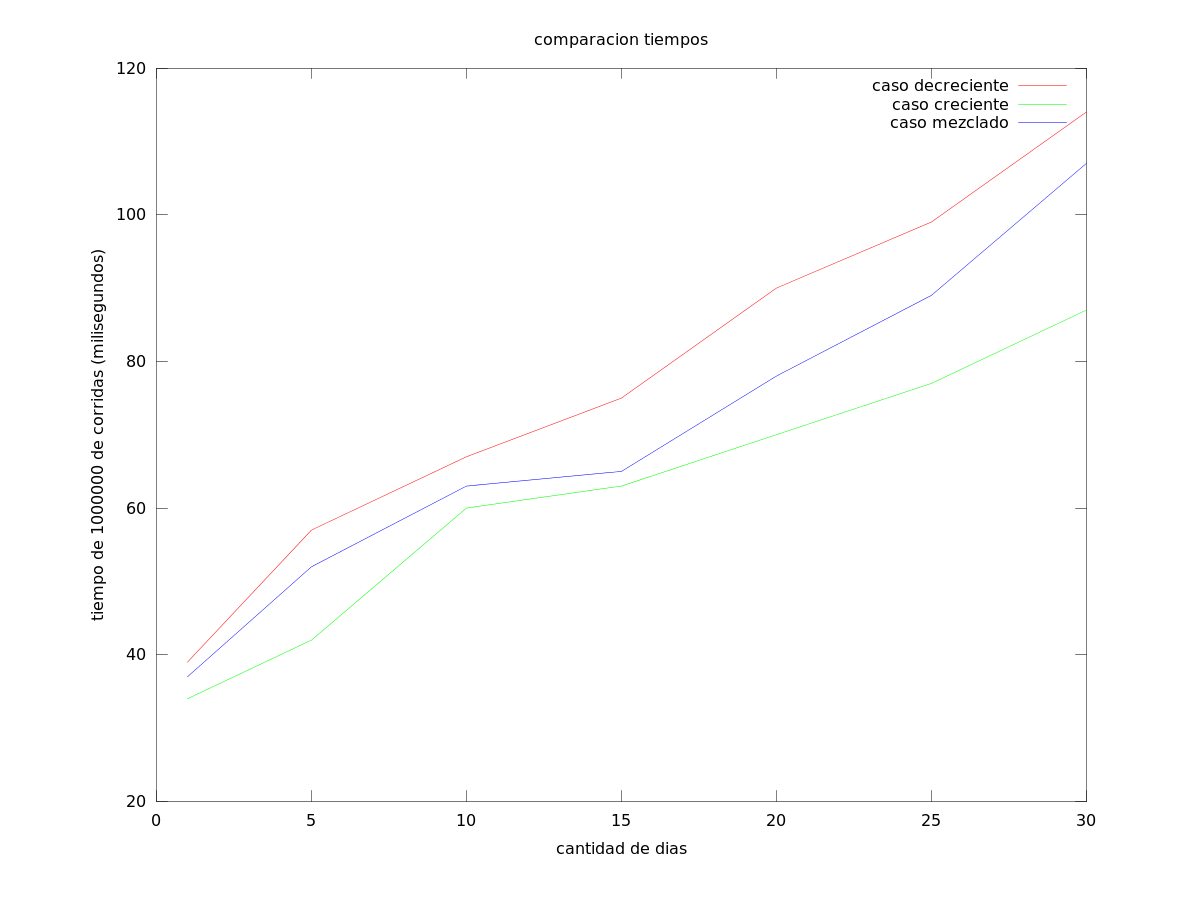
\includegraphics[width=340pt]{./figs/p1Tiempos.png}
\end{figure}


\indent Viendo el gráfico, podemos comprobar la complejidad del algoritmo. Se ve que los tiempos tienen un comportamiento lineal como el esperado. También se puede observar que el peor caso es en el que los números son decrecientes, dado que como vimos en la parte de complejidad, es el caso que mas asignaciones y comparaciones hace. El caso en el que los números son crecientes, lo podemos observar como el mejor caso (linea verde) y como era de esperarse, un caso en el que los números no tienen un patrón definido, cae entre medio de los casos mencionados anteriormente. \\



\clearpage

%%%%%%%%%%%%%%%%%%%%%%%%%%%
%					PROBLEMA 2					%
%%%%%%%%%%%%%%%%%%%%%%%%%%%

\section{Problema 2}

\subsection{Resolución}

\subsubsection{Explicación del problema}
\indent El objetivo de este ejercicio es, dada un red de amistades y 2
investigadores, determinar cuántas veces el entusiasmo que se genera en uno de
ellos se verá fraccionado hasta, finalmente, generar un cierto entusiasmo en el
otro. \\
\indent Esto sucederá sólo en aquellos casos en los cuales estos investigadores
tengan amigos en común. En caso de existir varias redes de amistades
(entendiendose por red de amistad a una conexión de amistades entre ambos
investigadores, sin que haya investigadores repetidos), se debe estudiar el caso
de la más corta, ya que esta red será la que generará el entusiasmo en el
investigador antes que cualquier otra y con la mayor proporción. \\
\indent Si no existiesen amigos en común entre ellos, es decir, si no existe una
red de amistad entre ambos, entonces el entusiasmo generado en uno nunca llegará
al otro, es decir la fracción de entusiasmo que le generará al investigador
destinatario será cero o, como se ha establecido, se indicará con $0$ la
cantidad de veces que éste se verá fraccionado.

\subsubsection{Primeros intentos de solución}
\indent En una primera aproximación al problema, pensamos en aplicar el
concepto de matrices de incidencia,
teniendo como índices a los investigadores por un lado y a las amistades por el
otro.\\
\indent Este clase de solución nos parecía productiva ya que al utilizar una
matriz, tanto para rellenarla en su totalidad como para recorrerla, los
algoritmos tienen una complejidad lineal O($m*n$), con $m$= cantidad de
amistades y $n$=cantidad de investigadores, quedando en evidencia que dicha
implementación cumplía la cota de complejidad pedida. \\
\indent Esta solución fue descartada una vez ya empezada su implementación.
Luego de buscar alguna estructura adecuada para representar a la matriz,
decidimos utilizar un diccionario de clave investigador y significado Lista de
amigos.\\
\indent El problema surgió a la hora de pensar un algoritmo para recorrer las
amistades con algún criterio y que no repita ninguna amistad. Luego de
contemplar varias opciones para tratar de solucionar este problema, nos dimos
cuenta de que estaba mal pensado el problema, ya que la matriz carecía de toda la
información relevante necesaria para realizar el algoritmo del recorrido de la
misma. Incluso sabiendo qué amistad se había recorrido, era dificil establecer
un criterio de recorrido que nos diera el largo de la red de amistades más corta
que conecta a 2 investigadores (luego explicamos por qué nos interesa ésta red
en particular \footnote{ver Aplicación de BFS}.

\subsubsection{BFS}
El algortimo de búsqueda BFS (por sus siglas en inglés, Breadth-First Search)
consiste en que dado un grafo $G= (V,E)$ y un vértice distinguido $s$, computa
la distancia (mínimo camino entre dos vértices) desde $s$ hasta cualquier
vértice que tenga algún camino simple que lo conecte con $s$.\\
\indent El algoritmo recorre un vértice, lo analiza y luego realiza el mismo
procedimiento con sus vértices adyacentes. Con el fin de no analizar 2 veces el
mismo vértice y así trabajar sólo con caminos mínimos,el algoritmo BFS setea los
vértices con distintos colores:

\begin{itemize}
\item \textit{blanco}: el análisis de vértices no abarcó este vértice en ninguna
instancia.
\item \textit{gris}: para indicar si ya ha sido encontrado y guardado en una
cola para, posteriormente, realizar el análisis de sus vértices adyacentes.
\item \textit{negro}:para indicar que ya se han guardado todos sus vértices
adyacentes para su posterior análisis.
\end{itemize}

El procedimiento BFS va construyendo un árbol BF que tiene cómo raíz a
$s$, como hijos directos de este a todos sus adyacentes, como hijos de esos a
sus respectivos hijos, y así sucesivamente.\\
\indent De esta forma, se crea una relación de orden entre los vértices, orden
establecido por la distancia al vértice $s$ que posee cada uno. Así todos
aquellos nodos que estén a distancia uno de $s$, estarán en el nivel 1 del árbol
BF.\\

\subsubsection{Aplicación de BFS al problema}
\indent \Obs{\textit{Estudiando los casos de tests provistos por la cátedra, 
pudimos observar que, cuando existen más de dos redes de amigos que conectan a
ambos investigadores,
el criterio para elegir una red de amigos, a través de la cuál 
se propaga el entusiasmo, es la que está conformada por la de menor cantidad de
investigadores.} }\\

\indent Antes que nada, realizamos el modelado del problema de esta forma:
Tomamos un grafo genérico $G(V,E)$, donde $V$ es el conjunto de vértices (aka
investigadores) de $G$ y $E$ un conjunto de pares de vértices(aka amistad entre
2 investigadores) , indicando las aristas que unen a dichos vértices en $G$.\\

\indent Dada una red de amigos, para saber cuántas veces se fracciona a la mitad
el entusiasmo del investigador $v_1$ hasta que recibe una porción de este el
investigador $v_n$, asumiendo que $v_1$ y $v_n$ tienen una red que los conecta,
tenemos la siguiente caracterización:
\begin{itemize}
 \item Si $v_1$ es amigo de $v_n$, entonces $v_n$ recibe la mitad del entusiasmo
de $v_1$, 
 ya que esta se divide a la mitad una sola vez y, a su vez, existe una única
arista en el camino que conecta a ambos.
 \item Si no son amigos, entonces cada uno de los amigos de $v_1$ reciben la
mitad del entusiasmo de $v_1$. Asumamos que $v_n$ se encuentra a distancia $n-1$
de $v_1$ y tomemos el único amigo de $v_1$, siendo este uno de los vértices del
camino mínimo que une a $v_1$ con $v_n$, al que llamaremos $v_2$. \\ 
\indent\indent Entre $v_1$ y $v_2$ hay una arista ($v_2$ se encuentra a
distancia 1 de $v_1$) y el entusiasmo de $v_1$ se fracciona una sola vez. Ahora,
entre $v_2$ y su amigo $v_3$, siendo este uno de los vértices del camino mínimo
que une a $v_1$ con $v_n$, entre $v_2$ y $v_3$ hay una arista ($v_3$ se
encuentra a distancia 1 de $v_2$). Entonces, entre $v_3$ y $v_1$ hay 2 aristas
($v_3$ se encuentra a distancia 2 de $v_1$) y el entusiasmo de $v_1$ se
fracciona una vez más que para $v_2$, es decir el entusiasmo de $v_1$ se
fracciona 2 veces hasta llegar a $v_3$. \\
\indent\indent Generalizando, para cualquier amigo $v_k$, con 2 $\leq$ k $\leq$
n:
 \begin{itemize}
  \item entre $v_k$ y $v_1$ hay k-1 aristas, es decir, se encuentran a distancia
k-1;
  \item el entusiasmo de $v_1$ se fracciona k-1 veces hasta llegar a $v_k$, y 
 \end{itemize}
\end{itemize}
\indent\indent Entonces, la cantidad de veces que se fracciona el entusiasmo de
$v_1$ hasta llegar a $v_n$ 
 es equivalente a la cantidad de aristas que exiten entre esos 2, es decir la
distancia entre ellos que es n-1.
 Es por esto que pudimos establecer la resolución del problema mediante
el uso del algortimo BFS, ya que la cantidad de fracciones que se produce sobre
el entusiasmo de $v_1$ hasta que genera algún nivel de entusiasmo en $v_n$, es
equivalente a calcular la distancia desde $v_1$ hasta $v_n$, que es lo que
calcula el BFS.\\

\indent Teóricamente, si la red de amigos en común más corta que
une $v_1$ con $v_n$ tiene un longitud $\delta$($i_1$,$v_n$) y $v_1$ se
entusiasma en un valor medible $e$,
luego $v_n$ se
entusiasmará con un nivel
\Gather{e' = \frac{e}{2.\delta(v_1,v_n)}.}

\indent Nuestra implementación trabaja con listas de adyacencia. Cada
investigador tiene asociada una lista donde están almacenados sus amigos (los
vértices adyacentes). Además, los investigadores poseen un campo estado que
puede tener alguno de los siguientes valores:

\begin{itemize}
\item \textit{no encontrado}: sería el equivalente al color blanco del algoritmo
de BFS, indicando que el recorrido del análisis de las amistades jamás abarcó
éste investigador. Inicialmente todos los investigadores están seteados
en este estado.
\item \textit{encontrado}: sería el equivalente al color gris del algoritmo de
BFS, indicando que ya se ha guardado este investigador en una cola para,
posteriormente, realizar el análisis sobre sus amistades.
\item \textit{visitado}: sería el equivalente al color negro del algoritmo de
BFS, indicando que ya se han guardado todos sus vértices adyacentes para su
análisis.
\end{itemize}

\hspace{-0.5cm}La función BFS realiza los siguientes pasos:
\begin{enumerate}
 \item Setea el estado del investigador fuente $s$ en gris.
 \item Encola $s$ en una cola vacía $c$.
 \item Desencola $c$ y ese elemento se almacena en $i$.
 \item Encola en $c$ los amigos de $i$.
 \item Setea el estado de $i$ en negro.
 \item Repite desde el paso 3 hasta que la cola quede vacía.
\end{enumerate}

\indent Una vez visitados todos los investigadores, se tiene como
postcondición que a todos se les ha seteado la distancia a $s$. En caso de que
no existiera un camino hacia $s$, la distancia por defecto no se modifica.\\ 
\indent El resultado de la función es el campo distancia del investigador
destinatario en caso de existir un camino entre él y $s$, o 0 en caso
contrario.\\
\indent Es importante notar que los investigadores se encolan y desencolan una
sola vez, ya que una vez encolados se los marca como "encontrado", y una vez
desencolado se los marca como "visitado", evitando así que en otra iteración se
los vuelva a encolar.

\subsubsection{Pseudocódigo}

\indent Para resolver el problema, utilizamos una función  llamada BFS \footnote{Es una adaptación del modelo en: Cormen, Thomas... [et al]; \textit{Introduction to Algorithms}, Cambridge, MIT Press, 2009; (p\'ag. 595)}
, que toma
2 datos de tipo investigador. donde investigador es una clase que posee la
siguiente información sobre el investigador:
\begin{itemize}
	\item nombre
	\item estado (no encontrado, encontrado, visitado)
	\item lista de amistades directas
	\item distancia al vértice desde el cuál se quiere calcular la distancia
\end{itemize}
\indent La función que resuelve el problema propiamente dicho, se llama BFS, y
se encuentra dentro de la clase relaciones. Esta clase contiene:
\begin{itemize}
\item una lista de todos los investigadores.
\item un investigador fuente.
\item un investigador destino.
\end{itemize}

\begin{algorithm}
\caption{BFS (\textbf{in/out} source,destination: \textsl{Investigador}) $\rightarrow$ res: \textsl{int}}
\begin{algorithmic}[1]

\STATE $source.estado \leftarrow encontrado$
\STATE $source.distancia \leftarrow 0$
\STATE $cola \leftarrow \emptyset$
\STATE $encolar(cola,source)$
\WHILE{$cola \neq \emptyset$}
	\STATE $actual \leftarrow desencolar(cola)$
	\FORALL{$v \in amigos(actual)$}
		\IF{$v.estado == no encontrado$}
			\STATE $v.estado \leftarrow encontrado$
			\STATE $v.distancia \leftarrow actual.distancia + 1$
			\STATE $encolar(cola,v)$
		\ENDIF
	\ENDFOR
	\STATE $actual.estado \leftarrow visitado$
\ENDWHILE
\IF{$destination.distancia == \infty$}
	\RETURN $0$
\ELSE
	\RETURN $destination.distancia$
\ENDIF
\end{algorithmic}
\end{algorithm}

\subsection{Complejidad}
\subsubsection{Análisis de complejidad}
\indent Analizamos el código de la función BFS línea por línea, siguiendo los
siguientes criterios:
\begin{itemize}
 \item Asignar valores enteros o chars acotados y comparar chars acotados
 tienen complejidad O(1). Los chars que comparamos son acotados por la
 longitud de ''no encontrado'' que es 13, ya que solo se
 comparan 3 strings posibles: ''encontrado'', ''visitado'' y ''no encontrado'', y
 el más largo es este último
 \item Pedir alguna de las variables del tipo Investigador tiene una complejidad
$O(1)$, 
 ya que se puede acceder a estas directamente.
 \subitem La función constructora del tipo Investigador tiene una complejidad 
 O($|$nombre$|$)+O($|$estado$|$)+O(crear una lista vacia)+O(pedir max value)=
 O(1)+O(1)+O(crear una lista vacia)+O(1)= O(crear una lista vacia) ;
 ya que los nombres de los investigadores y los strings que indican el estado
 son strings acotados por el más largo, que sabemos que será finito, por ende
toman O(1), y
 pedir el max value toma O(1)
 \item Las funciones del tipo genérico ''Queue''tienen la siguiente complejidad:
 \subitem crear una cola= O(crear lista enlazada)= O(1)
 \subitem ver si es vacía= O(1)
 \subitem encolar= O(1)
 \subitem desencolar= O(1)
 \item Las funciones del tipo genérico
''ArrayList''\footnote{http://docs.oracle.com/javase/6/docs/api/, java.utils,
ArrayList}  tienen
 la siguiente complejidad:
 \subitem crear iterador sobre ella = O(1)
 \subitem pedir el elemento de un índice= O(1)
 \subitem ver si hay siguiente= O(1)
 \subitem avanzar el iterador= O(1)
 
\end{itemize}

\indent Dado que estas son las únicas funciones que utilizamos en el código de
la función BFS, todas las líneas tienen complejidad O(1)\\
\indent Sólo falta analizar cuántas veces iteran los 2 whiles, para saber la 
complejidad de los mismos\\

%ESTO PARA ABAJO CAMBIA SI ALGUNA DE LAS FUNCIONES DENTRO DEL WHILE NO TOMA O(1)
\indent La complejidad del while más grande está determinada por la cantidad de
veces que itera 
y cada iteración toma O(cantidad de iteraciones del while anidado), es por esto
que
primero realizaremos el análisis del while anidado.\\

\indent El while anidado itera la lista de adyacencia de cada investigador $i$,
entonces
el while iterará $a_i$ veces, donde $a_i$ es el largo
de la lista de adyacencia de $i$.\\

\indent Ahora podemos determinar la complejidad del while más abarcativo. Como
habíamos
establecido antes, la complejidad de este será 
\Gather{O(cantidad\ de\ veces\ que\ itera) * O(cantidad\ de\ veces\ que\ itera\
el\ while\ anidado)}

\indent Este ciclo iterará hasta que la cola $c$ quede vacía. $C$ es la cola
donde se irá guardando
sólo una vez los investigadores. Entonces esta cola no quedará vacía hasta que
se haya encolado y desencolado 
a todos los investigadores de ella. Por ende, este while itera tantas veces como
investigadores haya.\\

\indent Además, por cada iteración, este while toma una complejidad O($a_i$),
donde $a_i$ es el largo
de la lista de adyacencia de $i$, que es el
investigador que se ha desencola ni bien se entra en el while. Como este while
itera una vez para cada investigador,
la complejidad que tomará finalmente será 
\Gather{O(k*(\sum_{i=1}^{k}(a_i)))} donde k es la cantidad de investigadores.

\indent Observar que la sumatoria, representa a la suma del largo de la lista de
adyacencia de cada investigador, ya que en cada iteración del while se recorre
la lista de adyacencia de un investigador y esto se realiza una única vez para
todo investigador, entonces su resultado es 
\Gather{O(\sum_{i=1}^{k}(a_i))= O(2a)}
siendo $a$ la cantidad de amistades total. Esto se debe a que se recorre 2 veces cada
amistad (una vez por cada investigador involucrado),pero como 2 es una
constante, no afecta
en la complejidad temporal de la función. Luego, tenemos que:
\Gather{O(\sum_{i=1}^{k}(a_i))= O(a)}
Luego la complejidad de la función BFS es 
\Gather{O(k)*O(a) = O(cantidad\ de\ investigadores)*O(cantidad\ de\ amistades)}

\subsection{Análisis de casos de test}

\clearpage

%%%%%%%%%%%%%%%%%%%%%%%%%%%
%					PROBLEMA 3					%
%%%%%%%%%%%%%%%%%%%%%%%%%%%

\section{Problema 3}

\subsection{Primeras Consideraciones}

En un temprano intento por resolver este problema diseñamos un procedimiento que buscara el punto medio del list\'on considerado y tomara como corte \'optimo en ese instante aquel que se ubicara lo m\'as cerca del punto medio. Si bien esta idea distaba de ser correcta para el problema (se tardar\'ia un tiempo en detectar que uno de los casos de test romp\'ia este modelo), nos permiti\'o acercarnos a la idea de resolverlo mediante recursi\'on. En definitiva, la funci\'on deb\'ia tomar un liston de largo \textit{n} y un conjunto de cortes dentro de ese rango, para luego elegir uno mediante la decisi\'on explicada y luego llamar recursivamente sobre los listones \textit{$n_1$} y \textit{$n_2$}, determinados al realizar el corte, junto con los conjuntos de cortes correspondientes a cada rango. Visto de esta manera, se trataba de un enfoque \textit{Divide \& Conquer} en que la soluci\'on se ir\'ia construyendo al ir concatenando en una lista los cortes elegidos en cada llamada de la funci\'on.

\indent Pronto identificar\'iamos el err\'oneo an\'alisis de la situaci\'on y, al detectar que se trataba de un problema de optimizaci\'on un tanto m\'as complejo, acudir\'iamos a la t\'ecnica de \textit{\textsl{Programaci\'on Din\'amica}}, bajo la cual modelamos e implementamos el problema, tal como se describe a continuaci\'on. \footnote{El an\'alisis de modelado y resoluci\'on del problema mediante PD ha sido tomado y adaptado del libro: Cormen, Thomas... [et al]; \textit{Introduction to Algorithms}, Cambridge, MIT Press, 2009; (p\'ags. 359 - 390)}


\subsection{Estructura de Permutaci\'on \'Optima}

Como se ha mencionado, los parámetros de este problema son un listón de largo $n$ y un conjunto de cortes $C$ ordenados de menor a mayor, tal que además $\#C = m$.  Dejando la consideración de costo de lado, una solución a este problema estría dada por una permutación del orden de los cortes que se quieren realizar, con lo cual en principio nos encontramos con $m!$ soluciones posibles. Sin embargo, dado que cada corte conlleva un costo $q$ igual al largo del listón en que se realiza, buscamos aquella permutación tal que al realizar los cortes en ese orden la sumatoria de costos sea la mínima posible.\\
\indent Para tratar de caracterizar la solución, llamamos $Q^{s}_{ij}$ ($0 \leq i \leq j < m$) al costo de realizar en orden los cortes $c_i$,$c_{i+1}$,...,$c_j$ en un listón de tamaño $s$. El caso trivial en que $i=j$, este costo será igual a $s$. En cambio, cuando $i < j$, se debe elegir algún orden para realizar los cortes, ya que de esto dependerá cuánto costará cada uno.\\
\indent De esto último se desprende que a la hora de evaluar el costo de un conjunto de cortes, siempre debemos elegir un corte pivot $c_k$ $(i \leq k < j)$ que determina dos secciones del listón a las que quedan asociados dos conjuntos disjuntos de cortes. Luego, para determinar $Q^{s}_{ij}$ en el caso no trivial:
			\begin{itemize} \itemsep -2pt
			\item \textbf{Primero} elegimos $k / i \leq k < j$
			\end{itemize}
			\begin{itemize} \itemsep -2pt
			\item \textbf{Luego} computamos $Q^{c_k}_{ik}$
			\end{itemize}
			\begin{itemize} \itemsep -2pt
			\item \textbf{Además} computamos $Q^{s-c_k}_{k+1j}$
			\end{itemize}
			\begin{itemize} \itemsep -2pt
			\item \textbf{Finalmente} sumamos ambos costos al de haber realizado $c_k$, el cual resulta ser $s$
			\end{itemize}

A partir de este modelado salta a la vista que la solución se construye recursivamente. Habiendo determinado esto, debemos ver si entonces se cumple el \textsl{Principio de Optimalidad}.\\
\indent Supongamos que encontramos el valor mínimo de $Q^{s}_{ij}$ tomando como corte pivot $c_k$ para algún $k$ entre $i$ y $j$. Luego por lo expuesto antes necesariamente el valor de la subsolución $Q^{c_k}_{ik}$ del subproblema deberá ser óptimo, ya que si existiera otro orden para obtener un costo más barato, entonces la solución inicial no habría sido la óptima. Lo mismo sucede al considerar el subproblema derecho. El absurdo proviene de que $Q^{s}_{ij} = Q^{c_k}_{ik} + s + Q^{s-c_k}_{k+1j}$, luego si la solución es óptima la suma de los términos que la conforman también debe serlo, lo cual se traduce en que las subsoluciones de los subproblemas determinados sean también óptimas.\\
\indent Se ve entonces que cualquier instancia no trivial del problema de optimización de los cortes requiere que se separe el problema en dos subproblemas, y que a partir de la óptima resolución de ellos podemos construir una solución óptima a nuestro problema. Es importante notar que se deben recorrer todos los posibles cortes pivot en una instancia dada para asegurarse que se eligió cortar de manera óptima.\\

\subsection{Solución Recursiva}

Para este problema podemos determinar la solución óptima recursivamente al ir combinando soluciones óptimas de los subproblemas determinados. En particular, se debe organizar el orden de los cortes en el listón en función de su costo. Es decir que la función que implementamos toma decisiones en base a esta variable, pero el objetivo ulterior no es devolver el costo final sino cierta permutación de cortes asociada a ese costo. Para ello entonces operamos también con una lista donde iremos agregando los cortes desde el primero al últimoq ue se realiza.\\

\indent Sea $P[i,j,s]$ la permutación de cortes asociada al valor óptimo $Q^{s}_{ij}$, luego la solución del problema estará dada por $P[0,m-1,s]$. La lista $P$ la definimos recursivamente de la siguiente manera:
			\begin{itemize} \itemsep -2pt
			\item Si $i = j$ el problema es trivial, pues sólo se realiza un corte en el listón s, con lo cual $P[i,j,s] = \{c_i\}$.
			\end{itemize}
			\begin{itemize} \itemsep -2pt
			\item Si $i < j$ debemos seguir lo expuesto antes y pensar que primero se realiza el corte pivot y luego se realizan 				los cortes de manera óptima sobre el sublistón izquierdo y de la misma manera sobre el sublistón derecho. Notar que 				es indistinto el orden en que se ponga el bloque izquierdo o derecho. De esta manera $P[i,j,s] = \{c_k\} ++ P[i,k,c_k] 				++ P[k+1,j,s-c_k]$.
			\end{itemize}

Sin embargo este modelo de recursión asume que se conoce cuál es el corte pivot que garantiza la solución óptima. En realidad, ese k debe ser elegido en función de la permutación que genere el mínimo costo. Como complemento a lo anterior llamamos $Q[i,j,s]$ al mínimo costo al realizar los cortes $c_i$ hasta $c_j$ en el listón de tamaño $s$, el cual también se define recursivamente de la siguiente manera:
	\[ Q[i,j,s] = \left\{ \begin{array}{ll}
		 s & \mbox{if $i = j$};\\
		\min_{i \leq k < j} \{ Q[i,k,c_k] + Q[k+1,j,s-c_k] \} + s & \mbox{if $i < j$}.\end{array} \right. \] 

	
Aunque se trate de dos funciones recursivas distintas, se podrá observar que están intimamente ligadas. En términos implementativos se trata simplemente de una sola función que evalúa costos y en vez de devolver este retorna la permutación de cortes que utilizó para llegar al mismo.\\

\indent Otra observación que debe hacerse es que en este análisis se pasó por alto el hecho de que, al seccionar el listón, estas funciones teóricas sólo recuerdan el tamaño, pero no los extremos relativos a las posiciones desde donde fue seccionado el listón original. De esta manera, en este análisis teórico estaríamos evaluando realizar el corte $c_i = 7$ en un listón cuyos extremos son 0 y 3 pero que ubicado en el listón original sus extremos serían 5 y 8. Esta omisión se da ya que sólo volvería engorroso el planteo de las funciones, pero desde ya es algo que sí se contempla en la función implementada.

\subsection{Calculando las Subsoluciones}

¿Qué sucede a la hora de calcular las diversas subsoluciones de los subproblemas que se van planteando? Hasta aquí sólo se ha modelado una forma recursiva para resolver el problema, teniendo en cuenta que éste cumple el principio de optimalidad. ¿Pero acaso es esto mejor que la fuerza bruta, o backtracking, donde podríamos evaluar todas las permutaciones posibles? La respuesta es, por el momento, no. En la Figura ~\ref{fig:overl} vemos un esquema del árbol de problemas que se va generando al evaluar el modelo recursivo antes descripto, llamando a $P[1,4,s]$. Se puede ver fácilmente como en diversos llamados de la función recursiva se repiten los subproblemas, lo cual implica que la función planteada hasta el momento debe resolver varios cómputos repetidas veces. Esta característica, \textsl{superposición de subproblemas}, es esencial para una solución de Programación Dinámica. A diferencia de un problema que se pudiera resolver con Divide \& Conquer, en que se generan nuevos y disjuntos subproblemas, aquí 
vemos como en realidad el espacio de subproblemas distintos es reducido.\\
\begin{figure}[h]
\centering                                                       
        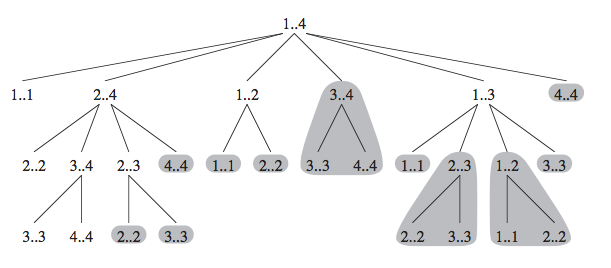
\includegraphics[width=320pt]{./figs/p3overlapping.png}
	\caption{Se ve la superposición de subproblemas, y como los pintados en gris serían buscados en una tabla y no calculados. \textsl{Fuente: Cormen..., p(385)}. }
	\label{fig:overl}
\end{figure}
\indent Es posible ver que implementar directamente una solución basada en el modelo tal cual fue planteado hasta aquí tomaría tiempo exponencial respecto de $m$ \footnote{Si bien escapa a nuestro foco de análisis, puede encontrarse una demostración para el análogo problema de producto de matrices en \textit{Cormen...} (p. 386)}. Es así que el último ingrediente agregado a este modelo es una tabla o diccionario que recordará aquellos subproblemas calculados para que en caso de requerir una solución precomputada esté disponible en tiempo constante. De esta manera nuestra solución al problema es un algoritmo recursivo, \textsl{top down} ya que va partiendo los problemas grandes en subproblemas más pequeños, pero que a diferencia de la ineficiente versión original va 'recordando' o \textsl{memoizando} las soluciones para que otras ramas de las llamadas recursivas no tengan que recalcular lo mismo nuevamente. Más adelante, en el análisis de complejidad de nuestro algoritmo, se verá cuán importante es la mejora 
al introducir la \textsl{memoización} en términos de tiempo de cómputo (no así de memoria).

\subsection{Estructuras}

Antes de analizar el algoritmo implementado y evaluar su complejidad, es importante realizar un breve análisis de las estructuras usadas para la resolución del problema.\\

\textbf{Listón.} Decidimos crear la estructura Listón para así tener alojados no sólo los datos iniciales del problema (lista de cortes, tamaño) sino también la tabla de soluciones (parciales en la mayor parte de los casos) computadas a lo largo de la ejecución. De esta manera contenemos toda la información en un mismo objeto al que se accede y se modifica en las distintas llamadas de la recursión, mientras que lo único que cambia en las mismas es el pasaje de los parámetros que determinan qué sublistones se mirarán dentro de ese listón (esto se analiza luego en la función correspondiente).\\
\indent Los campos de Listón: el tamaño es un entero, mientras que los cortes se guardan en un arreglo. El diccionario de soluciones no es otra cosa que una matriz o tabla. Dado que los métodos de Listón, salvo el constructor, son simplemente acceder a estos campos, se ve sin dificultad que tienen complejidad $O(1)$. En cambio, el constructor debe crear la matriz e inicializar la mitad de ella con el valor $\infty$ para indicar que todavía no se han insertado soluciones en esos casilleros. Por lo tanto, la complejidad del mismo es $O(m^2)$. El significado del contenido de la tabla y el por qué de cómo está indexada se ve a continuación.\\

\textbf{Solución.} Esta estructura es una tupla, con la semántica de una 'solución' al problema. La definimos de esta manera ya que como primera componenete tiene un costo, y como segunda una lista (implementada sobre la interfaz de Java \textsl{List$<T>$} sobre la clase \textsl{ArrayList$<T>$}). El vínculo entre ambas componentes es que el costo corresponde a haber realizado los cortes de la lista, en ese orden, en algún sublistón. A diferencia del modelo teórico planteado antes, aquí no guardamos ninguna relación con el tamaño del listón. Esto es porque en realidad el valor de $Q^{s}_{ij}$ es único en función de $i$ y $j$; nunca se dará una situación en que se quiera calcular $Q^{s}_{ij}$ y $Q^{t}_{ij}$ con $ s \neq t$. Por ello, la tabla de 'memoización' está indexada en base a los índices de corte $i,j$, y en definitiva es por ello que se produce la mencionada superposición de subproblemas.\\
\indent La complejidad de ambos constructores es constante. Por un lado el constructor vacío \textit{Solucion()} se trata de una asignación de un campo entero y la creación de un ArrayList vacío, lo cual crea una lista en base a un arreglo con capacidad para 10 elementos. Por el otro lado, el constructor que toma dos enteros realiza también una asignación a un campo y además de crear una lista vacía, le agrega el otro entero de la entrada (lo cual es, amortizado, O(1)).\\
\indent Por último, esta clase tiene otra operación llamada \textit{Combinar(Solucion,Solucion,int,int)}. Si llamamos $s1$ y $s2$ a las soluciones de entrada, entonces la complejidad de esta operación es O($max$($\#$s1.cortes, $\#$s2.cortes)), ya que luego de crear la lista vacía, primero agrega el corte individual que vino en la entrada, y luego agrega (concatena) los cortes de s1, para luego agregar los de s2. Dado que agregar $n$ elementos demanda O($n$), la complejidad estará por la máxima cantidad de cortes que se encuentre entre las dos soluciones. Si tenemos en cuenta que se trata de subconjuntos de la cantidad de cortes inicial, la complejidad de peor caso de esta operación será O($m$).\footnote{Las complejidades de las clases de Java fueron tomadas de http://docs.oracle.com/javase/6/docs/api/}

\subsection{Pseudocódigos y Complejidades}

\begin{algorithm}
\caption{cortarListon (\textbf{in/out} liston: \textsl{Liston}) $\rightarrow$ res: \textsl{Solucion}}
\begin{algorithmic}[1]

\STATE $ m \leftarrow liston.cantCortes()$
\STATE $ solucion \leftarrow memoizedCosto(liston,0,m-1,0,liston.largo()$
\RETURN $solucion$

\end{algorithmic}
\end{algorithm}

\begin{algorithm}
\caption{memoizedCosto (\textbf{in/out} liston: \textsl{Liston}, \textbf{in} i,j,izq,der: \textsl{int}) $\rightarrow$ res: \textsl{Solucion}}
\begin{algorithmic}[1]

\IF{ $i == j$}
	\IF{ $liston.dameCorte(i) == izq || liston.dameCorte(j) = der$ }
		\STATE $corteInvalido \leftarrow Solucion()$
		\STATE $liston.insertarSolucion(i,j,corteInvalido)$
		\RETURN $corteInvalido$
	\ELSE
		\STATE $corteBase \leftarrow Solucion(der-izq, liston.dameCorte(i))$
		\STATE $liston.insertarSolucion(i,j,corteBase)$
		\RETURN $corteBase$
	\ENDIF
\ELSE
	\STATE $costoAnt \leftarrow \infty$
	\FOR{$k = i$ \textbf{to} $j-1$} 
		\IF{ $not(liston.haySolucion(i,k)$}
			\STATE $memoizedCosto(liston,i,k,izq,liston.dameCorte(k))$
		\ENDIF
		\STATE $solIzq \leftarrow liston.dameSolucion(i,k)$
		\IF {$not(liston.haySolucion(k+1,j)$}
			\STATE $memoizedCosto(liston,k+1,j,liston.dameCorte(k),der)$
		\ENDIF
		\STATE $solDer \leftarrow liston.dameSolucion(k+1,j)$
		\STATE $costoAct \leftarrow solIzq.costo + solDer.costo + (der-izq)$
		\IF {$costoAct < costoAnt$}
			\STATE $costoAnt \leftarrow costoAct$
			\STATE $ktemp \leftarrow k$
			\STATE $sol_ij \leftarrow combinar(solIzq,solDer,costoAct,ktmp)$
		\ENDIF
	\ENDFOR
	\STATE $liston.insertar(i,j,sol_{ij})$
	\RETURN $sol_{ij}$
\ENDIF
\end{algorithmic}
\end{algorithm}

\indent La primera función, \textsl{cortarListon}, hereda su complejidad de \textsl{memoizedCosto}, ya que la instrucción de la primera línea es simplemente O(1).\\
\indent La complejidad de \textsl{memoizedCosto} es un tanto más compleja de calcular, ya que se trata de una función recursiva. Supongamos por el momento que es $T(m)$. La propuesta para este análisis es primero hacer un desglose de las complejidades de cada línea, y luego ver de qué manera repercute esto en la recursión y cuál es finalmente la verdadera complejidad de la función.\\
\indent Si dividiéramos en bloques la función, el primero estaría comprendido entre la línea 1 y la línea 10, representando el análisis de casos base. Todas las operaciones en este bloque, por lo justificado en la sección anterior sobre los métodos de las estructuras, es O(1).\\
\indent El segundo bloque, el cual va de la línea 12 a la 28, comprende casi la mayor parte de la función, y es el que se ocupa de verificar qué corte se debe realizar en esa llamada, actualizar la tabla de memoización y devolver una solución parcial. Salvo una asignación en O(1) al principio, el resto del bloque está comprendido por un sub-bloque iterativo. Supongamos que la complejidad de lo que se ejecuta en ese bloque es $T(F)$. Luego, como el ciclo itera entre $i$ y $j$, y estos a su vez están comprendidos entre $0$ y $m-1$, la complejidad de este bloque sería O($m * T(F)$). Ahora bien, veamos cuál es la complejidad dentro del ciclo.\\
\indent Aquí es donde se produce el truco de la memoización, que nos ahorrará operar en tiempo exponencial (como se mostró antes) para llegar, idealmente y según veremos en pocas líneas, a tiempo polinomial. Tanto en las líneas 14-17, como 18-21, la función parte en el listón en el $k$-ésimo corte y luego busca en la tabla los costos de lo que queda a izquierda y a derecha. Si nunca lo calculó, deberá hacerlo mediante la recursión. Supongamos para el análisis que siempre encuentra la solución en la tabla. Entonces, hasta aquí, la complejidad dentro del ciclo es constante. Luego hace algunas cuentas con enteros y comparaciones, para en la línea 26 utiliza el método combinar, que según probamos en las estructuras demanada O($m$). De esta manera, con la suposición de que siempre encuentra los valores en la tabla, la complejidad del ciclo es O($m * m$), o sea O($m^2$). Finalmente la penúltima línea inserta la solución parcial en tiempo constante y la devuelve.\\
\indent Suponiendo que los valores pedidos siempre están en la tabla (se acceden entonces en O(1)), llegamos a que $T(m) = O(m^2)$. Pero la realidad es que nuestra suposición no es del todo correcta, ya que al menos hay $m$ casos en los que para esos cortes se deben computar los subproblemas izquierdo y derecho por primera vez, con lo cual en realidad la complejidad es O($m * m^2$), lo que \textbf{finalmente da en el orden de} O($m^3$).

\subsection{Análisis Toma de Tiempos}

\indent Para correr el algoritmo, hicimos 1000 corridas de cada caso para poder tener un tiempo estimativo en milisegundos, dado que si corrìamos una sola vez los casos, el tiempo era insignificante (para poca cantidad de cortes).\\
\indent A continuacion presentamos el grafico obtenido para un liston de tamaño 200 variando el parámetro $m$ (cant. de cortes) entre 3, 6, 10, 15, 19, 27 y 36:

\begin{figure}[h]
\centering                                                       
        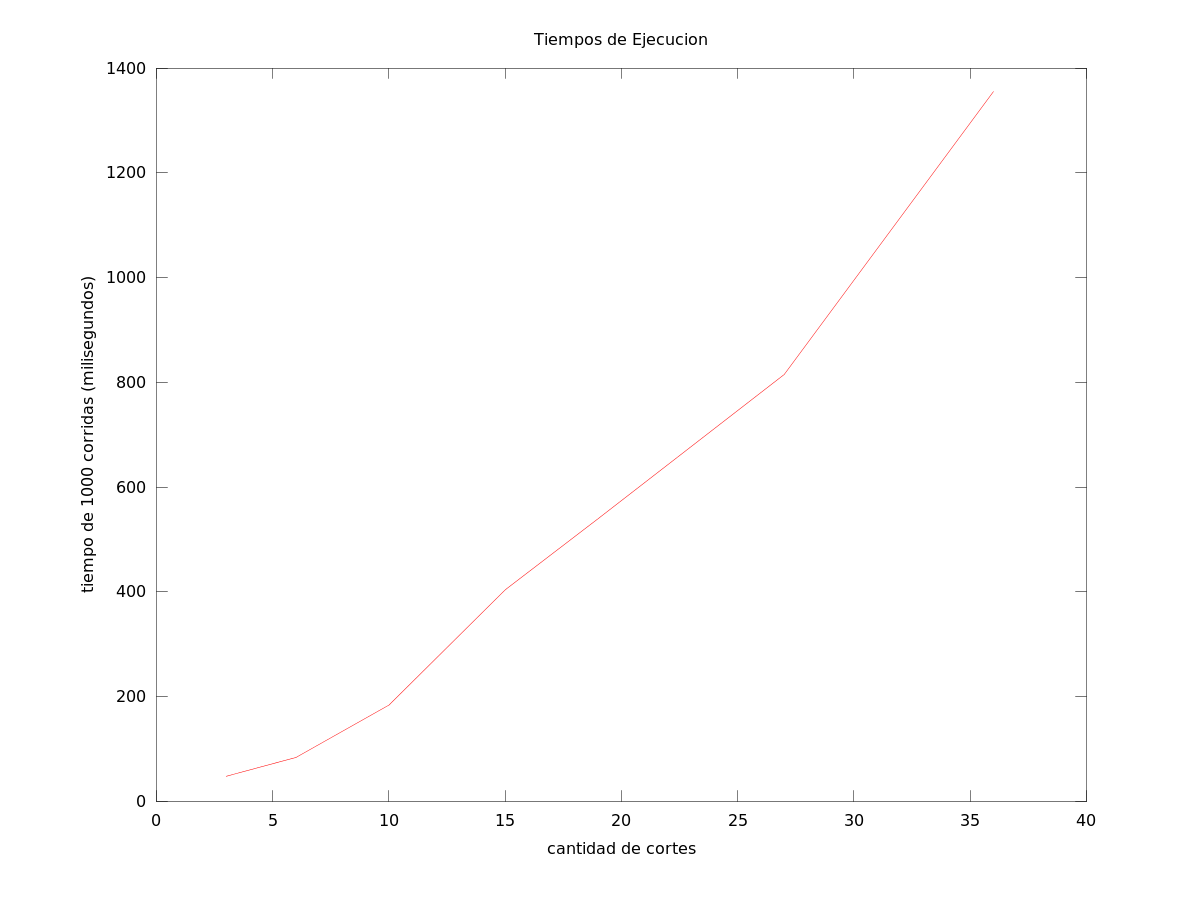
\includegraphics[width=320pt]{./figs/p3tiempos.png}
	\caption{En este gráfico se ejemplifican algunas corridas para cierta cantidad de cortes}
	\label{fig:p3tiempos}
\end{figure}

\indent Al realizar el gràfico, nos llevamos la sorpresa de que la gràfica resultante parecìa no ser cúbica. Luego de realizar varias pruebas notamos que el comportamiento de los tiempos que obteníamos no era tan regular como esperábamos (a diferencia por ejemplo del primer problema). Si bien no sabemos con certeza a qué atribuirlo, algunas de las hipótesis con que contamos es que la metodología para contar los tiempos no fuera la correcta, o que no hubieramos dispuesto una distribución uniforme de los casos de prueba. Esto es, si bien variamos el parámetro $m$, desconocemos qué relación puede existir con la longitud del listón. Si bien por el modelado y el análisis expuesto esto no infiere directamente, podría ser que lo haga la densidad o distribución de cortes dada la superficie del listón.\\

\clearpage

%%%%%%%%%%%%%%%%%%%%%%%%%%%
%					referencias					%
%%%%%%%%%%%%%%%%%%%%%%%%%%%

\section{Referencias}

\subsection{Fuentes teoricas}
\indent Clases Teóricas, Practicas y de Laboratorio de Algoritmos y Estructuras de Datos III.\\
\clearpage

\end{document}
